
\subsection{Kleuren} \label{Kleuren}
Het onderscheiden en detecteren van verschillende kleuren speelt een belangrijke rol bij het detecteren van schermen. De waarneming van een kleur aan de hand van een foto stemt echter niet altijd overeen met de afgebeelde kleur op een scherm. De voornaamste oorzaken hiervan zijn lichtinval en reflectie. Tijdens detectie moet er dus rekening gehouden worden met deze factoren. De keuze van de kleurruimte zal hierbij essentieel zijn om een goede range op te stellen voor detectie van de verschillende kleuren.

\subsubsection{Kleurmodellen en ruimtes}
Door de jaren heen zijn veel verschillende modellen ontwikkeld om het visuele lichtspectrum weer te geven. Al deze modellen hebben hun voordelen en nadelen en worden dan ook voor verschillende doeleinden gebruikt. De meest voorkomende modellen zijn RGB, CIE en HSL/HSV. 
\paragraph{RGB} is een additief kleurmodel waarbij een kleur wordt beschreven aan de hand van de drie primaire kleuren: rood, groen en blauw. Elke kleur wordt gevormd aan de hand van een combinatie van deze drie kleuren. RGB wordt heel veel gebruikt in grafische toepassingen. Wanneer een foto door een computer wordt uitgelezen zal dit ook in RGB-waarden gebeuren. Alleen zal dit model niet gebruikt kunnen worden voor detectie aangezien het model een niet-lineaire en discontinue ruimte vormt. Deze discontinuïteit maakt het beschrijven van een verandering in tint moeilijk. Daarnaast is het RGB-model gevoelig aan verandering van licht, wat resulteert in een verandering van tint. 
\paragraph{CIE} is gemaakt door de Commission Internationale de l'Éclairage (CIE). Het was het eerste model dat kleuren wiskundig kan voorstellen. Hierbij wordt gebruik gemaakt van de link tussen de verschillende golflengtes van het visueel spectrum en de manier waarop mensen kleuren waarnemen. Het CIE-model lag ook aan de basis van bijna alle andere kleurmodellen die achteraf ontwikkeld zijn. Het grootste nadeel van het gebruik van dit model is de complexe omzetting van RGB naar CIE. Om deze reden wordt dit model niet gebruikt voor de detectie.  
\paragraph{HSL en HSV} maken allebei deel uit van het cylindrisch model. Deze worden beschreven in drie dimensies: een hoek, die de tint voorstelt gaande van 0\degree (rood), naar 120\degree (groen), richting 240\degree (blauw), om uiteindelijk bij 360\degree (rood) rond te zijn (zie figuur \ref{colorWheel}). Een horizontale dimensie, die de saturatie beschrijft en een verticale dimensie, die de lichtheid (HSL) of waarde (HSV) bepaalt. Het voornaamste voordeel en de reden voor het gebruik van deze modellen over RGB en CIE is het feit dat deze modellen imuun zijn aan veranderingen in licht. Want deze zitten in een aparte dimensie. Een ander voordeel is de continue tint in de HSV- en HSL-modellen. HSL wordt uiteindelijk boven HSV verkozen door zijn symmetrie voor licht en donker. \cite{inbook} \cite{rasouli2017effect}

\begin{figure}[H]
	\center
	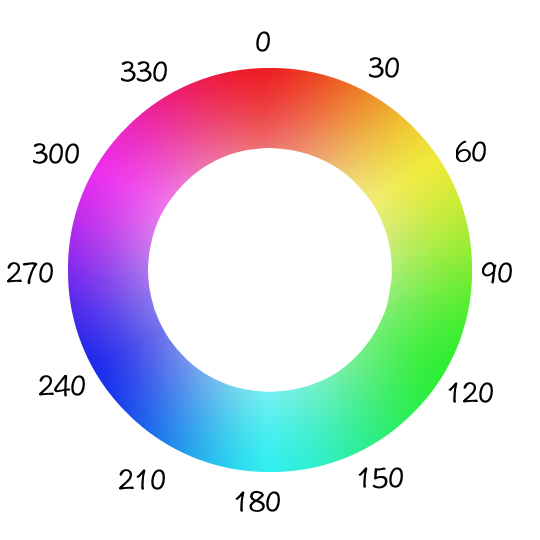
\includegraphics[width=0.6\textwidth]{img/hslColorWheel.png}
	\caption{De waarden van de verschillende tinten in HSL. \cite{hslColorWheel}}
	\label{colorWheel}
\end{figure}

\subsubsection{Ranges in de HSL kleurruimte} \label{Ranges}
Naast de keuze van het kleurmodel, HSL, moeten ook de kleuren voor detectie bepaald worden. Uiteindelijk heeft onze gebruikte methode zes verschillende kleuren nodig om te detecteren. De keuze is gegaan naar de drie basiskleuren (rood, groen en blauw) aangevuld met de kleuren, die theoretisch het verst van elkaar verwijderd liggen op de cirkel (cyaan, magenta en geel). Bijgevolg liggen de gekozen kleuren allemaal op 60\degree  \space van elkaar verwijderd. Vervolgens werd voor elke kleur een range bepaald onder verschillende omstandigheden. Hiervoor zijn foto's genomen van verschillende schermen in verschillende lichtomstandigheden en reflecties met verschillende camera's. Deze foto's dienen als dataset om de range van elke kleur te bepalen. Elke pixel van een foto werd uitgelezen en nadien omgezet van een RGB-waarde naar een HSL-waarde. Deze HSL-waarden zijn vervolgens geplot in functie van tint en saturatie, alsook in functie van tint en lichtheid, zie figuur \ref{hslPlot}. De bekomen scatterplots toonden telkens een geconcentreerd gebied van datapunten aan dat aan de hand van lineaire functies begrensd werd. Deze lineaire functies worden dan gebruikt als range om de kleur te detecteren. Dit werd voor alle zes kleuren uitgevoerd. Zie appendix \ref{kleurenPlots} voor alle gemaakte plots. \cite{TSAI20121291}

\begin{figure}[H]
	\center
	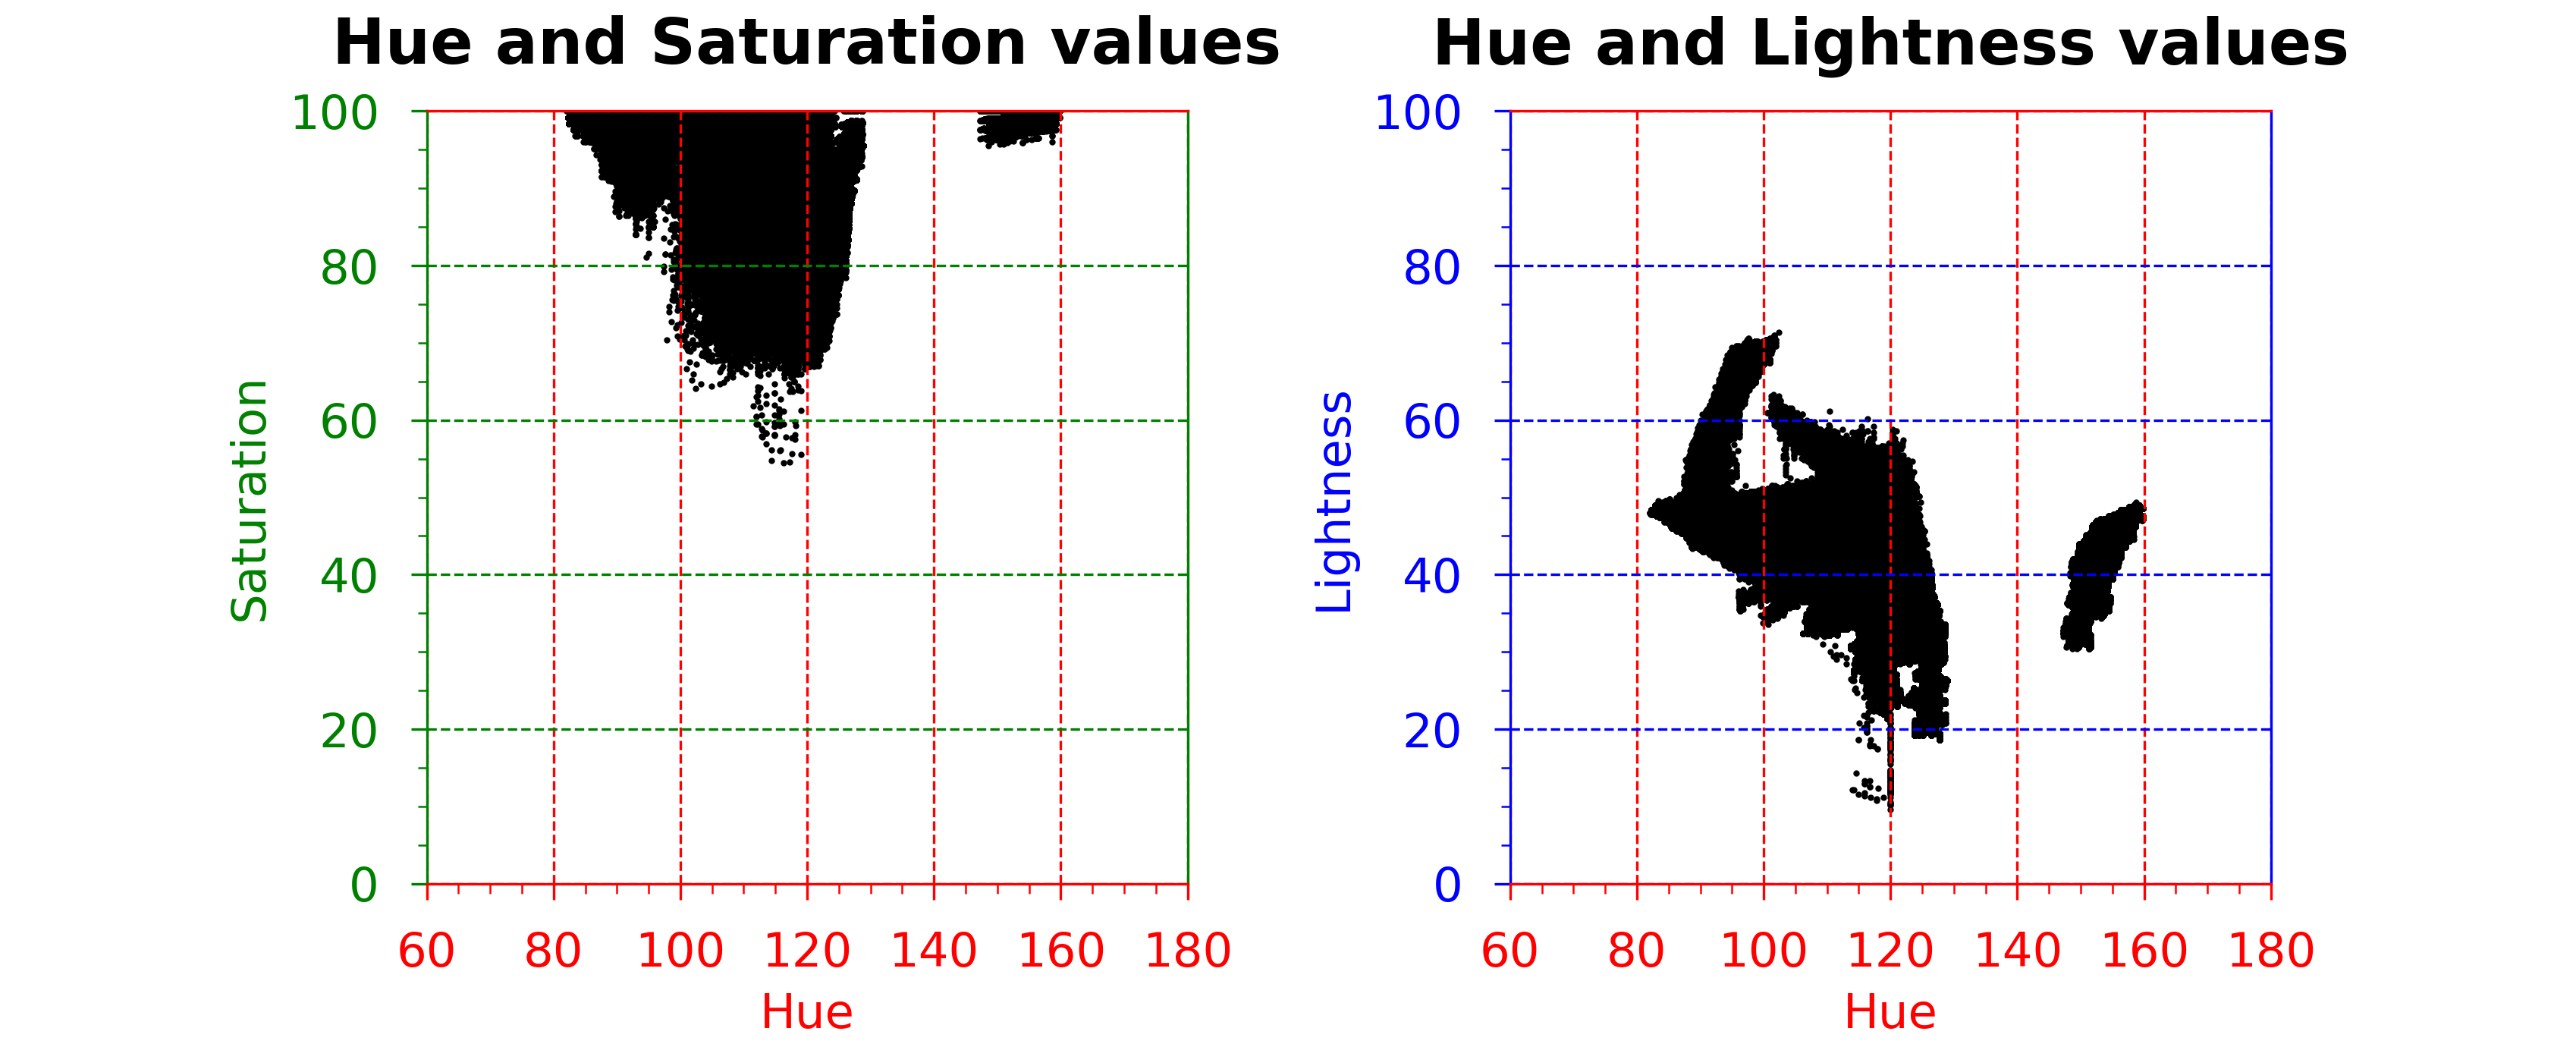
\includegraphics[width=\textwidth]{img/hslGreen.png}
	\caption{Scatter plots in functie van tint en saturatie, alsook in functie van tint en lichtheid voor de kleur groen.}
	\label{hslPlot}
\end{figure}

\subsubsection{Verdere verbeteringen} \label{Verbeteringen kleur}
Uit de plots is echter gebleken dat aparte onderscheiding van zes verschillende kleuren geen goede optie is door overlap van de ranges van de verschillende kleuren. Dit is het gevolg van zeer verschillende waarnemingen van een kleur naargelang de omstandigheden waarin een foto getrokken wordt. Het is dus niet mogelijk om zes verschillende kleuren correct te onderscheiden in alle omstandigheden. Nieuwe methodes moeten gevonden worden waar niet zoveel verschillende kleuren van elkaar onderscheiden moeten worden. Een eerste mogelijkheid is om een detectie uitgaande van slechts drie kleuren te verkiezen boven een detectie met zes kleuren. Bij het gebruik van een drie-kleuren-detectie zijn twee opties, waarbij de kleuren opnieuw zo ver mogelijk van elkaar verwijderd liggen (120\degree),  mogelijk. Enerzijds het gebruik van de kleuren rood, groen en blauw of anderzijds de kleuren cyaan, magenta en geel. De uiteindelijke keuze valt op rood, groen en blauw aangezien deze minder ver fluctueren van de theoretische waarde dan cyaan, magenta en geel. Aan deze optie wordt reeds gewerkt om de detectie te verbeteren. Daarnaast is het ook een optie om eerder relatief naar het contrast tussen kleuren te kijken in plaats van detectie op basis van absolute ranges. Ook deze optie wordt reeds bekeken om de identificatie te verbeteren.

\subsection{Flood fill}
Elk individueel slavescherm laat een vooraf bepaalde afbeelding zien met gekende kleur-waarden zoals op figuur \ref{scherm}. Deze afbeelding voor detectie is een combinatie van vorige iteraties van het project. Het combineren van een border met een kruis geeft het meeste informatie over de associatie van de kleur-gefilterde pixels bij overlap of afgedekte delen van het scherm en bovendien meer informatie over de relatieve oriëntatie van het scherm op de foto. Om deze schermen te detecteren wordt de foto gefilterd op basis van gekende HSL ranges (zie \ref{Ranges}) en een standaard four-way flood fill algoritme \cite{floodfill} om de associatie van de verbonden pixels te behouden. Na de executie van de flood fill is er voor elk gedetecteerd eiland een pixelmasker met een unieke ID per eiland opgeslagen in elke pixel, waar de verdere bewerkingen op uitgevoerd zullen worden. Het geimplementeerde floodfillalgoritme groeit volgens de vier pixel-buren en een stack-based iteratieproces om recursie-overflow tegen te gaan bij grote afbeeldingen en eilanden. In een worstcasescenario zal dit algoritme een eiland detecteren over de volledige afbeelding. Aangezien elke pixel maximaal vier keer in de stack terecht kan komen, door zijn vier buren, loopt deze flood fill volgens een tijdscomplexiteit van 
\[O(4mn)=O(mn)\]
 met m en n de dimensies van de afbeelding. De grootte van elk eiland zal in de praktijk over het algemeen een stuk kleiner zijn dan de volledige afbeelding. \\

\begin{figure}[H]
\centering
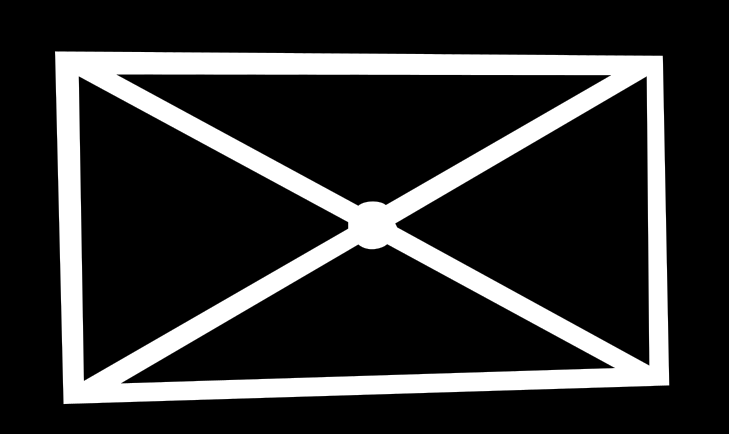
\includegraphics[scale=0.5]{img/mask.png}
\caption{Kleurenmasker van een scherm na floodfill}
\end{figure}

\noindent
Niet enkel de associatie van de gemaskeerde pixels wordt op deze manier behouden, maar deze methode maakt ook dat de komende pixelbewerkingen maar over een minimale bounding box uitgevoerd worden ten opzichte van de volledige pixelmatrix. Elk resulterend resultaat van floodfill geeft een verbonden pixelverzameling, een island, als resultaat. De resulterende islands worden achteraf gefilterd opdat elk eiland de drie kleuren van de border en het middelpunt bevatten. Als er aan deze voorwaarde voldaan is wordt er een poging gedaan om lokaal een middelpunt en geldige barcode te lezen \ref{barcode}. Bij het falen van een van deze verificatiestappen wordt het eiland verworpen, de overblijvende eilanden zijn geldige eilanden voor verdere hoekdetectie.

\subsection{Hoekpunten}
Er werd vooraf een algemeen hoek-detectiealgoritme Shi-Tomashi \cite{shi-tomashi} geïmplementeerd en getest, maar gaf een te complex resultaat op de binaire maskers om de juiste hoeken te filteren. Dit algoritme draagt ook een relatief grote overhead door de x- en y-sobeloperaties die elk een volledige pixel convolution over alle pixels als pre-processing toepassen. Onze algoritmes zijn veel simplistischer en zullen in de praktijk nooit verder dan de boundary van een eiland uitgevoerd worden in tegenstelling tot de volledige island matrix, maar geven een perfect bruikbaar resultaat voor onze noden.

In de eerste stap wordt er bepaald of het scherm voornamelijk recht of gekanteld is ten opzichte van de foto. Hiervoor wordt langs de linkerkant van het kader de standaarddeviatie van pixels in het masker berekend. Bij een standaardafwijking onder de 15\% wordt een scherm als liggend of verticaal gezien op de foto en niet gekanteld.\\
Als in eerste instantie het scherm als gedraaid beschouwd wordt, zal er vanuit elke rand van de bounding box van het eiland de eerste mask-pixel als corner beschouwd worden. In het geval dat het scherm relatief horizontaal of verticaal recht staat, zal er loodrecht op de randen gezocht worden (zie figuur: \ref{fig:perp search}), maar volgens een diagonaal tot een mask-pixel (zie figuur: \ref{fig:diag search}). Beide variante hoekdetectie algoritmes lopen in worst-case scenario volgens
\[O(4mn)=O(mn)\]
maar zoals eerder vermeld zullen deze in de praktijk maar tot de boundary van het masker lopen.

\begin{figure}[H] 
\centering
\begin{subfigure}{0.5\textwidth}
\centering
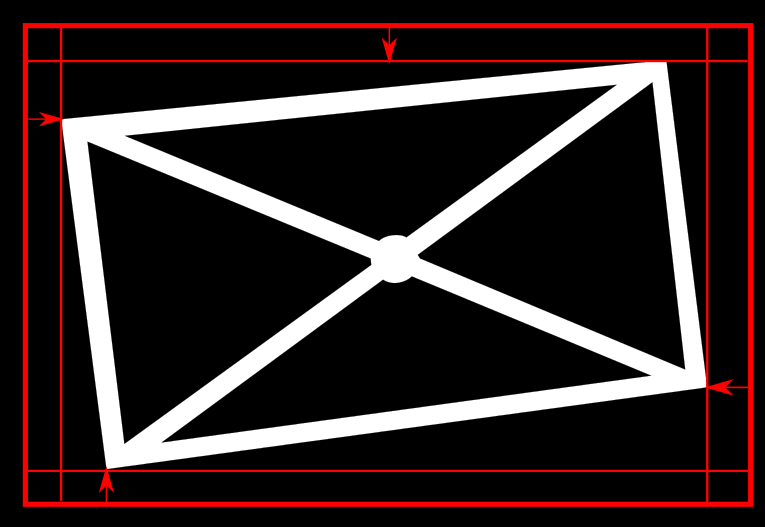
\includegraphics[width=0.9\textwidth]{img/perpSearch.png}
\caption{Loodrechte corner search}
\label{fig:perp search}
\end{subfigure}%
\begin{subfigure}{0.5\textwidth}
\centering
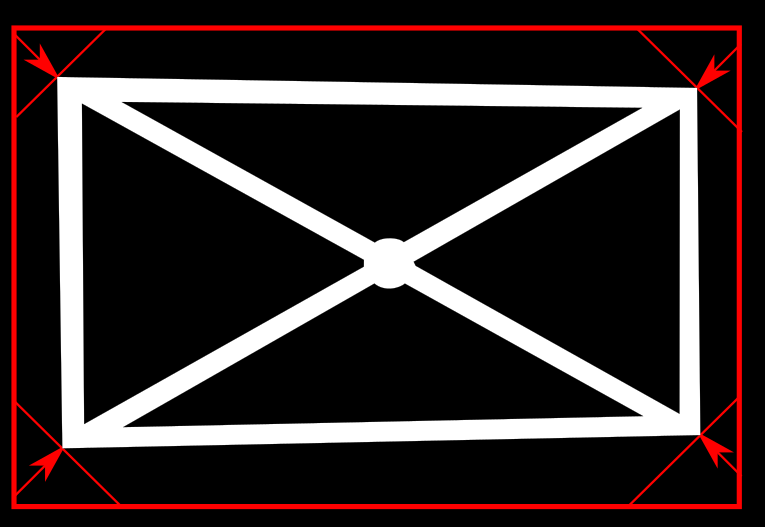
\includegraphics[width=0.9\textwidth]{img/diagSearch.png}
\caption{Diagonale corner search}
\label{fig:diag search}
\end{subfigure}
\caption{Hoekdetectie}
\end{figure}

\noindent
Beide variaties van hoek-detectie zullen altijd vier hoeken als resultaat opleveren. Dit zullen door overlap en foutjes in het maskeren niet altijd correcte hoeken zijn. Na het bepalen, worden de hoeken nagekeken of deze resultaten wel degelijk kwalificeren als hoek. Deze kwalificatie is gebaseerd op bepaalde eigenschappen die in de buurt van elke hoek moeten gevonden worden, namelijk twee lijnen die tot de boord behoren en een diagonaallijn die naar het middelpunt van het scherm loopt (zie figuur: \ref{fig:correcte hoek}). Deze lijnen zijn bepaald door te filteren door de border- en diagonaal-kleur die gescheiden zijn door een witte rand. Deze aanwijzingen moeten gevonden worden binnen een relatieve straal die gelijk is aan 25\% van de maximale afstand van de hoekpunten tot het middelpunt. Als in een eerder gevonden hoek deze voorwaarden niet aanwezig zijn (zie figuur: \ref{fig:foute hoek}), wordt deze hoek verworpen als resultaat van de hoekdetectie.

\begin{figure}[H] 
\centering
\begin{subfigure}{0.5\textwidth}
\centering
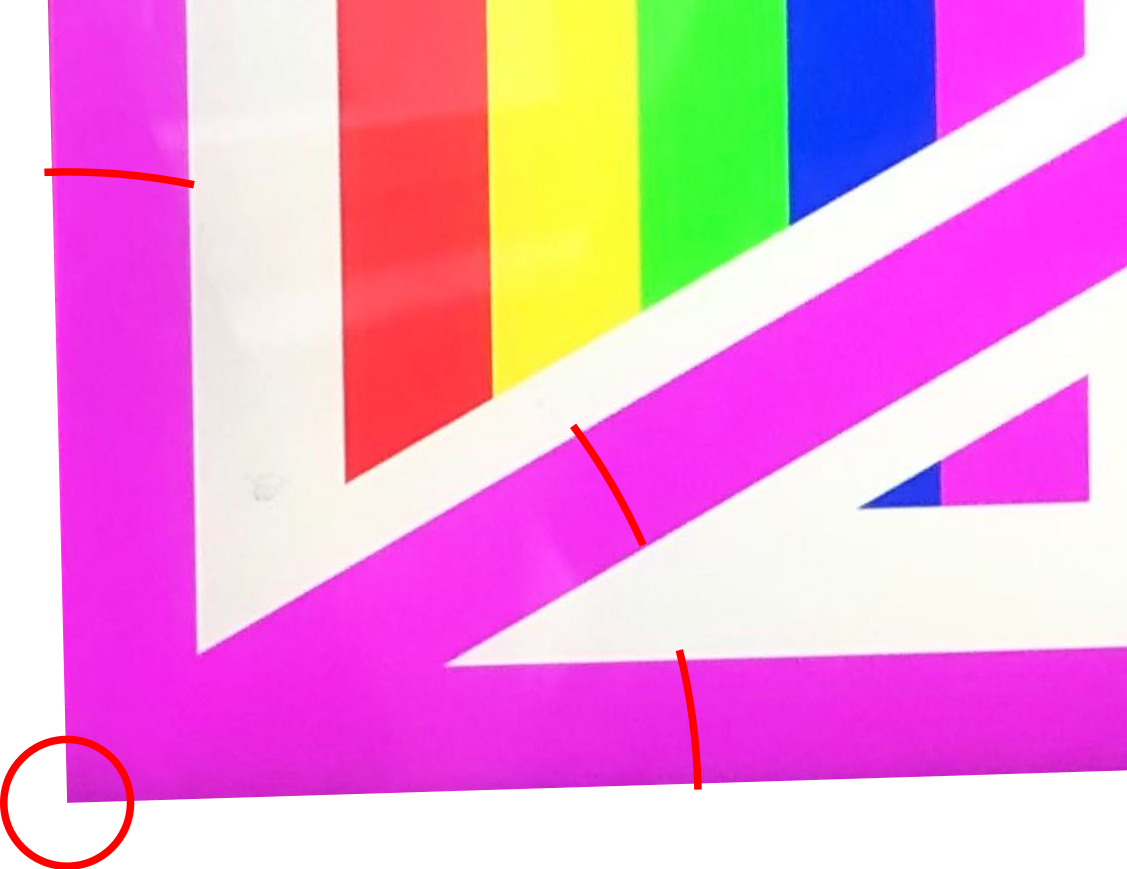
\includegraphics[width=0.6\textwidth]{img/correctCorner.png}
\caption{Een correcte hoek}
\label{fig:correcte hoek}
\end{subfigure}%
\begin{subfigure}{0.5\textwidth}
\centering
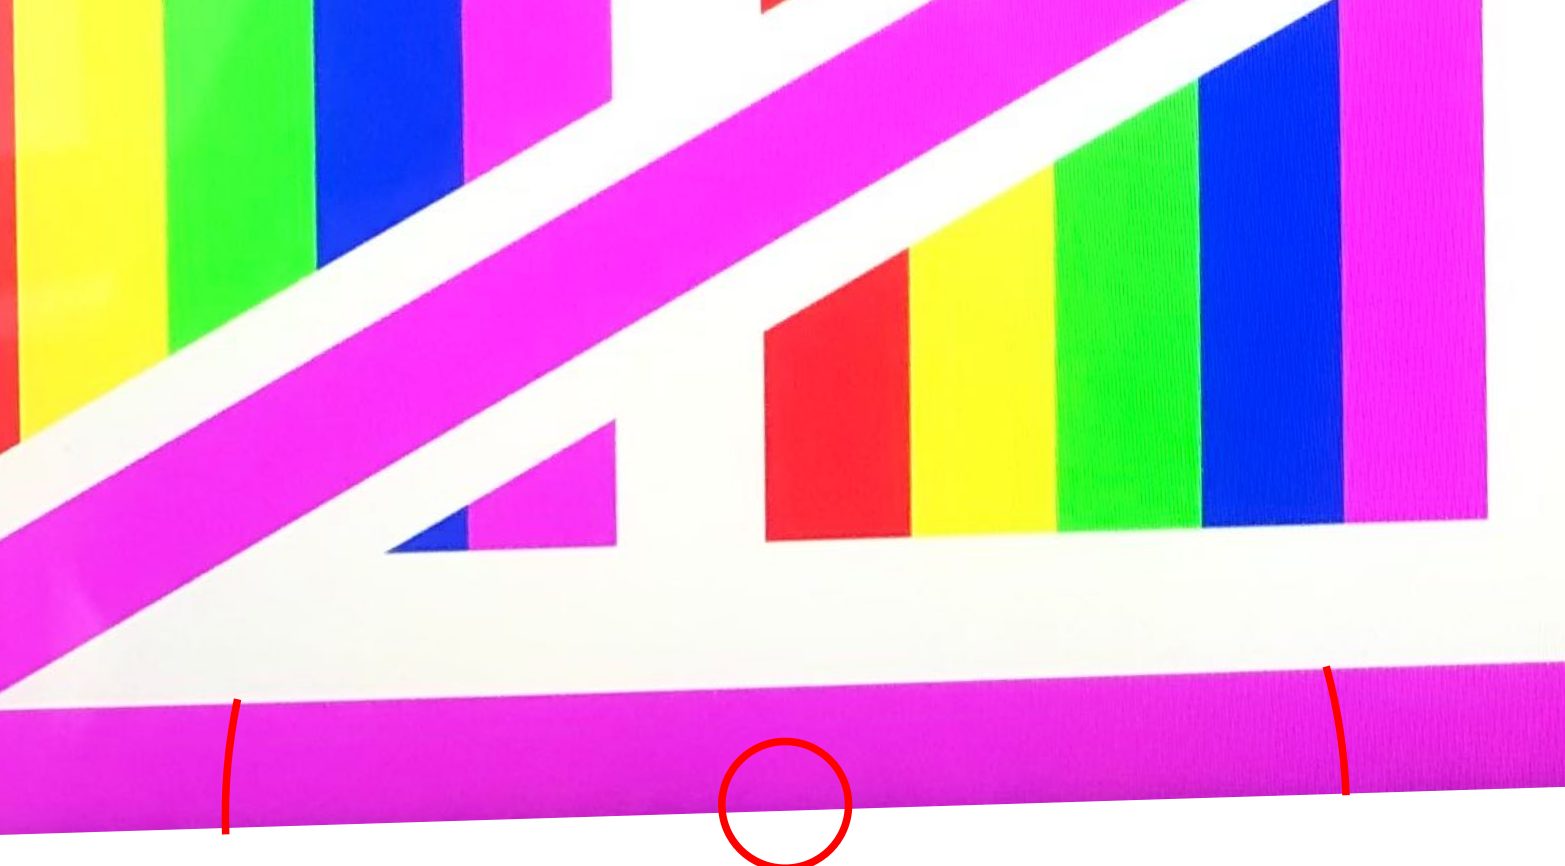
\includegraphics[width=0.6\textwidth]{img/notACorner.png}
\caption{Hoek zonder volledige features}
\label{fig:foute hoek}
\end{subfigure}
\caption{Hoekfiltering}
\end{figure}